\documentclass[twoside]{book}

% Packages required by doxygen
\usepackage{fixltx2e}
\usepackage{calc}
\usepackage{doxygen}
\usepackage[export]{adjustbox} % also loads graphicx
\usepackage{graphicx}
\usepackage[utf8]{inputenc}
\usepackage{makeidx}
\usepackage{multicol}
\usepackage{multirow}
\PassOptionsToPackage{warn}{textcomp}
\usepackage{textcomp}
\usepackage[nointegrals]{wasysym}
\usepackage[table]{xcolor}

% Font selection
\usepackage[T1]{fontenc}
\usepackage[scaled=.90]{helvet}
\usepackage{courier}
\usepackage{amssymb}
\usepackage{sectsty}
\renewcommand{\familydefault}{\sfdefault}
\allsectionsfont{%
  \fontseries{bc}\selectfont%
  \color{darkgray}%
}
\renewcommand{\DoxyLabelFont}{%
  \fontseries{bc}\selectfont%
  \color{darkgray}%
}
\newcommand{\+}{\discretionary{\mbox{\scriptsize$\hookleftarrow$}}{}{}}

% Page & text layout
\usepackage{geometry}
\geometry{%
  a4paper,%
  top=2.5cm,%
  bottom=2.5cm,%
  left=2.5cm,%
  right=2.5cm%
}
\tolerance=750
\hfuzz=15pt
\hbadness=750
\setlength{\emergencystretch}{15pt}
\setlength{\parindent}{0cm}
\setlength{\parskip}{3ex plus 2ex minus 2ex}
\makeatletter
\renewcommand{\paragraph}{%
  \@startsection{paragraph}{4}{0ex}{-1.0ex}{1.0ex}{%
    \normalfont\normalsize\bfseries\SS@parafont%
  }%
}
\renewcommand{\subparagraph}{%
  \@startsection{subparagraph}{5}{0ex}{-1.0ex}{1.0ex}{%
    \normalfont\normalsize\bfseries\SS@subparafont%
  }%
}
\makeatother

% Headers & footers
\usepackage{fancyhdr}
\pagestyle{fancyplain}
\fancyhead[LE]{\fancyplain{}{\bfseries\thepage}}
\fancyhead[CE]{\fancyplain{}{}}
\fancyhead[RE]{\fancyplain{}{\bfseries\leftmark}}
\fancyhead[LO]{\fancyplain{}{\bfseries\rightmark}}
\fancyhead[CO]{\fancyplain{}{}}
\fancyhead[RO]{\fancyplain{}{\bfseries\thepage}}
\fancyfoot[LE]{\fancyplain{}{}}
\fancyfoot[CE]{\fancyplain{}{}}
\fancyfoot[RE]{\fancyplain{}{\bfseries\scriptsize Generated by Doxygen }}
\fancyfoot[LO]{\fancyplain{}{\bfseries\scriptsize Generated by Doxygen }}
\fancyfoot[CO]{\fancyplain{}{}}
\fancyfoot[RO]{\fancyplain{}{}}
\renewcommand{\footrulewidth}{0.4pt}
\renewcommand{\chaptermark}[1]{%
  \markboth{#1}{}%
}
\renewcommand{\sectionmark}[1]{%
  \markright{\thesection\ #1}%
}

% Indices & bibliography
\usepackage{natbib}
\usepackage[titles]{tocloft}
\setcounter{tocdepth}{3}
\setcounter{secnumdepth}{5}
\makeindex

% Hyperlinks (required, but should be loaded last)
\usepackage{ifpdf}
\ifpdf
  \usepackage[pdftex,pagebackref=true]{hyperref}
\else
  \usepackage[ps2pdf,pagebackref=true]{hyperref}
\fi
\hypersetup{%
  colorlinks=true,%
  linkcolor=blue,%
  citecolor=blue,%
  unicode%
}

% Custom commands
\newcommand{\clearemptydoublepage}{%
  \newpage{\pagestyle{empty}\cleardoublepage}%
}

\usepackage{caption}
\captionsetup{labelsep=space,justification=centering,font={bf},singlelinecheck=off,skip=4pt,position=top}

%===== C O N T E N T S =====

\begin{document}

% Titlepage & ToC
\hypersetup{pageanchor=false,
             bookmarksnumbered=true,
             pdfencoding=unicode
            }
\pagenumbering{alph}
\begin{titlepage}
\vspace*{7cm}
\begin{center}%
{\Large My Project }\\
\vspace*{1cm}
{\large Generated by Doxygen 1.8.13}\\
\end{center}
\end{titlepage}
\clearemptydoublepage
\pagenumbering{roman}
\tableofcontents
\clearemptydoublepage
\pagenumbering{arabic}
\hypersetup{pageanchor=true}

%--- Begin generated contents ---
\chapter{File Index}
\section{File List}
Here is a list of all files with brief descriptions\+:\begin{DoxyCompactList}
\item\contentsline{section}{\hyperlink{draw_8cpp}{draw.\+cpp} }{\pageref{draw_8cpp}}{}
\item\contentsline{section}{\hyperlink{input_8cpp}{input.\+cpp} }{\pageref{input_8cpp}}{}
\item\contentsline{section}{\hyperlink{main_8cpp}{main.\+cpp} }{\pageref{main_8cpp}}{}
\item\contentsline{section}{\hyperlink{mainwindow_8cpp}{mainwindow.\+cpp} }{\pageref{mainwindow_8cpp}}{}
\item\contentsline{section}{\hyperlink{mainwindow_8h}{mainwindow.\+h} }{\pageref{mainwindow_8h}}{}
\item\contentsline{section}{\hyperlink{struct_8h}{struct.\+h} }{\pageref{struct_8h}}{}
\item\contentsline{section}{\hyperlink{threeD__to__ortho_8cpp}{three\+D\+\_\+to\+\_\+ortho.\+cpp} }{\pageref{threeD__to__ortho_8cpp}}{}
\item\contentsline{section}{\hyperlink{twoD__to3D_8cpp}{two\+D\+\_\+to3\+D.\+cpp} }{\pageref{twoD__to3D_8cpp}}{}
\end{DoxyCompactList}

\chapter{File Documentation}
\hypertarget{draw_8cpp}{}\section{draw.\+cpp File Reference}
\label{draw_8cpp}\index{draw.\+cpp@{draw.\+cpp}}
{\ttfamily \#include $<$math.\+h$>$}\newline
{\ttfamily \#include $<$Qt\+Core$>$}\newline
{\ttfamily \#include $<$Qt\+Gui$>$}\newline
{\ttfamily \#include \char`\"{}include/struct.\+h\char`\"{}}\newline
Include dependency graph for draw.\+cpp\+:
\nopagebreak
\begin{figure}[H]
\begin{center}
\leavevmode
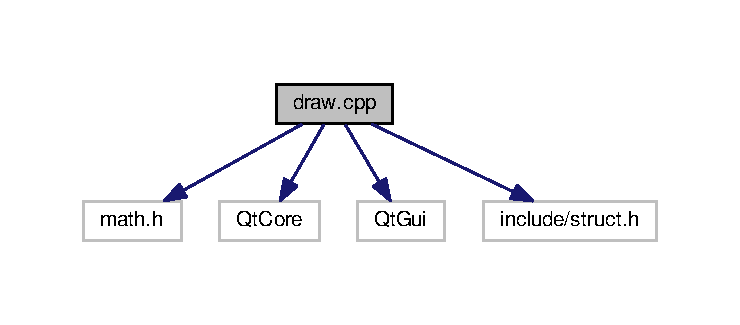
\includegraphics[width=350pt]{draw_8cpp__incl}
\end{center}
\end{figure}
This graph shows which files directly or indirectly include this file\+:
\nopagebreak
\begin{figure}[H]
\begin{center}
\leavevmode
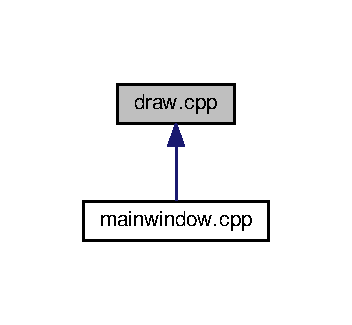
\includegraphics[width=169pt]{draw_8cpp__dep__incl}
\end{center}
\end{figure}
\subsection*{Functions}
\begin{DoxyCompactItemize}
\item 
three\+View \hyperlink{draw_8cpp_a969d6b40b0869b06f8cfded66c9b4719}{get\+\_\+three\+\_\+views} (string filename)
\item 
void \hyperlink{draw_8cpp_ab0fc9fff71b1111ac7a1430b062c0d9d}{print\+\_\+nodes} (vector$<$ node $>$ v)
\item 
void \hyperlink{draw_8cpp_a2ee335a43fbd0ba4663095611edd021d}{print\+\_\+edges} (vector$<$ edge $>$ v)
\item 
coordinate \hyperlink{draw_8cpp_a6b1da8a3461f46770e2c8666f32ebe51}{get\+\_\+average} (vector$<$ node $>$ v)
\item 
int \hyperlink{draw_8cpp_ac1a707c12c57b7cbf3ef84308a298acb}{get\+\_\+max\+\_\+y} (vector$<$ edge $>$ v)
\item 
int \hyperlink{draw_8cpp_aec887c68a3a59f16763fb16330e80185}{get\+\_\+max\+\_\+x} (vector$<$ edge $>$ v)
\item 
int \hyperlink{draw_8cpp_a15cf00bb6773d72a8a740ecce84ad95e}{get\+\_\+min\+\_\+x} (vector$<$ edge $>$ v)
\item 
int \hyperlink{draw_8cpp_a7337d85eb762ca8735b9be6520b25e62}{get\+\_\+min\+\_\+y} (vector$<$ edge $>$ v)
\item 
int \hyperlink{draw_8cpp_a911f1943b4548fcec0048ef7b786050e}{get\+\_\+min\+\_\+z} (vector$<$ edge $>$ v)
\item 
int \hyperlink{draw_8cpp_aa4c9ace07665494ea060c8b74a6fde2b}{get\+\_\+max\+\_\+z} (vector$<$ edge $>$ v)
\item 
Q\+Picture \hyperlink{draw_8cpp_a64dcf14345b66c2a69a13d8a374426de}{draw\+\_\+views} (vector$<$ edge $>$ v)
\item 
Q\+Picture \hyperlink{draw_8cpp_a7c3da4110b99906ffdeb8686942c0dda}{draw\+\_\+xy} (vector$<$ edge $>$ v)
\item 
Q\+Picture \hyperlink{draw_8cpp_a4efbb5676dd85c462f4f558a28af0893}{draw\+\_\+yz} (vector$<$ edge $>$ v)
\item 
Q\+Picture \hyperlink{draw_8cpp_a3105a48af84b6c7fadd10e7a5b7772c4}{draw\+\_\+xz} (vector$<$ edge $>$ v)
\end{DoxyCompactItemize}


\subsection{Function Documentation}
\mbox{\Hypertarget{draw_8cpp_a64dcf14345b66c2a69a13d8a374426de}\label{draw_8cpp_a64dcf14345b66c2a69a13d8a374426de}} 
\index{draw.\+cpp@{draw.\+cpp}!draw\+\_\+views@{draw\+\_\+views}}
\index{draw\+\_\+views@{draw\+\_\+views}!draw.\+cpp@{draw.\+cpp}}
\subsubsection{\texorpdfstring{draw\+\_\+views()}{draw\_views()}}
{\footnotesize\ttfamily Q\+Picture draw\+\_\+views (\begin{DoxyParamCaption}\item[{vector$<$ edge $>$}]{v }\end{DoxyParamCaption})}

Takes a graph as an input. Renders view from the same graph.\mbox{\Hypertarget{draw_8cpp_a7c3da4110b99906ffdeb8686942c0dda}\label{draw_8cpp_a7c3da4110b99906ffdeb8686942c0dda}} 
\index{draw.\+cpp@{draw.\+cpp}!draw\+\_\+xy@{draw\+\_\+xy}}
\index{draw\+\_\+xy@{draw\+\_\+xy}!draw.\+cpp@{draw.\+cpp}}
\subsubsection{\texorpdfstring{draw\+\_\+xy()}{draw\_xy()}}
{\footnotesize\ttfamily Q\+Picture draw\+\_\+xy (\begin{DoxyParamCaption}\item[{vector$<$ edge $>$}]{v }\end{DoxyParamCaption})}

Takes a graph description (vector of nodes) as and input. Draws the XY coordinates of this graph.\mbox{\Hypertarget{draw_8cpp_a3105a48af84b6c7fadd10e7a5b7772c4}\label{draw_8cpp_a3105a48af84b6c7fadd10e7a5b7772c4}} 
\index{draw.\+cpp@{draw.\+cpp}!draw\+\_\+xz@{draw\+\_\+xz}}
\index{draw\+\_\+xz@{draw\+\_\+xz}!draw.\+cpp@{draw.\+cpp}}
\subsubsection{\texorpdfstring{draw\+\_\+xz()}{draw\_xz()}}
{\footnotesize\ttfamily Q\+Picture draw\+\_\+xz (\begin{DoxyParamCaption}\item[{vector$<$ edge $>$}]{v }\end{DoxyParamCaption})}

Takes a graph description (vector of nodes) as and input. Draws the XZ coordinates of this graph.\mbox{\Hypertarget{draw_8cpp_a4efbb5676dd85c462f4f558a28af0893}\label{draw_8cpp_a4efbb5676dd85c462f4f558a28af0893}} 
\index{draw.\+cpp@{draw.\+cpp}!draw\+\_\+yz@{draw\+\_\+yz}}
\index{draw\+\_\+yz@{draw\+\_\+yz}!draw.\+cpp@{draw.\+cpp}}
\subsubsection{\texorpdfstring{draw\+\_\+yz()}{draw\_yz()}}
{\footnotesize\ttfamily Q\+Picture draw\+\_\+yz (\begin{DoxyParamCaption}\item[{vector$<$ edge $>$}]{v }\end{DoxyParamCaption})}

Takes a graph description (vector of nodes) as and input. Draws the YZ coordinates of this graph.\mbox{\Hypertarget{draw_8cpp_a6b1da8a3461f46770e2c8666f32ebe51}\label{draw_8cpp_a6b1da8a3461f46770e2c8666f32ebe51}} 
\index{draw.\+cpp@{draw.\+cpp}!get\+\_\+average@{get\+\_\+average}}
\index{get\+\_\+average@{get\+\_\+average}!draw.\+cpp@{draw.\+cpp}}
\subsubsection{\texorpdfstring{get\+\_\+average()}{get\_average()}}
{\footnotesize\ttfamily coordinate get\+\_\+average (\begin{DoxyParamCaption}\item[{vector$<$ node $>$}]{v }\end{DoxyParamCaption})}

Returns a coordinate average of the coordinates of all the nodes in a vector of nodes.\mbox{\Hypertarget{draw_8cpp_aec887c68a3a59f16763fb16330e80185}\label{draw_8cpp_aec887c68a3a59f16763fb16330e80185}} 
\index{draw.\+cpp@{draw.\+cpp}!get\+\_\+max\+\_\+x@{get\+\_\+max\+\_\+x}}
\index{get\+\_\+max\+\_\+x@{get\+\_\+max\+\_\+x}!draw.\+cpp@{draw.\+cpp}}
\subsubsection{\texorpdfstring{get\+\_\+max\+\_\+x()}{get\_max\_x()}}
{\footnotesize\ttfamily int get\+\_\+max\+\_\+x (\begin{DoxyParamCaption}\item[{vector$<$ edge $>$}]{v }\end{DoxyParamCaption})}

Helper function that gets maximum x coordinate of a node in a vector of edges.\mbox{\Hypertarget{draw_8cpp_ac1a707c12c57b7cbf3ef84308a298acb}\label{draw_8cpp_ac1a707c12c57b7cbf3ef84308a298acb}} 
\index{draw.\+cpp@{draw.\+cpp}!get\+\_\+max\+\_\+y@{get\+\_\+max\+\_\+y}}
\index{get\+\_\+max\+\_\+y@{get\+\_\+max\+\_\+y}!draw.\+cpp@{draw.\+cpp}}
\subsubsection{\texorpdfstring{get\+\_\+max\+\_\+y()}{get\_max\_y()}}
{\footnotesize\ttfamily int get\+\_\+max\+\_\+y (\begin{DoxyParamCaption}\item[{vector$<$ edge $>$}]{v }\end{DoxyParamCaption})}

Helper function that gets maximum y coordinate of a node in a vector of edges.\mbox{\Hypertarget{draw_8cpp_aa4c9ace07665494ea060c8b74a6fde2b}\label{draw_8cpp_aa4c9ace07665494ea060c8b74a6fde2b}} 
\index{draw.\+cpp@{draw.\+cpp}!get\+\_\+max\+\_\+z@{get\+\_\+max\+\_\+z}}
\index{get\+\_\+max\+\_\+z@{get\+\_\+max\+\_\+z}!draw.\+cpp@{draw.\+cpp}}
\subsubsection{\texorpdfstring{get\+\_\+max\+\_\+z()}{get\_max\_z()}}
{\footnotesize\ttfamily int get\+\_\+max\+\_\+z (\begin{DoxyParamCaption}\item[{vector$<$ edge $>$}]{v }\end{DoxyParamCaption})}

Helper function that gets maximum z coordinate of a node in a vector of edges.\mbox{\Hypertarget{draw_8cpp_a15cf00bb6773d72a8a740ecce84ad95e}\label{draw_8cpp_a15cf00bb6773d72a8a740ecce84ad95e}} 
\index{draw.\+cpp@{draw.\+cpp}!get\+\_\+min\+\_\+x@{get\+\_\+min\+\_\+x}}
\index{get\+\_\+min\+\_\+x@{get\+\_\+min\+\_\+x}!draw.\+cpp@{draw.\+cpp}}
\subsubsection{\texorpdfstring{get\+\_\+min\+\_\+x()}{get\_min\_x()}}
{\footnotesize\ttfamily int get\+\_\+min\+\_\+x (\begin{DoxyParamCaption}\item[{vector$<$ edge $>$}]{v }\end{DoxyParamCaption})}

Helper function that gets minimum x coordinate of a node in a vector of edges.\mbox{\Hypertarget{draw_8cpp_a7337d85eb762ca8735b9be6520b25e62}\label{draw_8cpp_a7337d85eb762ca8735b9be6520b25e62}} 
\index{draw.\+cpp@{draw.\+cpp}!get\+\_\+min\+\_\+y@{get\+\_\+min\+\_\+y}}
\index{get\+\_\+min\+\_\+y@{get\+\_\+min\+\_\+y}!draw.\+cpp@{draw.\+cpp}}
\subsubsection{\texorpdfstring{get\+\_\+min\+\_\+y()}{get\_min\_y()}}
{\footnotesize\ttfamily int get\+\_\+min\+\_\+y (\begin{DoxyParamCaption}\item[{vector$<$ edge $>$}]{v }\end{DoxyParamCaption})}

Helper function that gets minimum y coordinate of a node in a vector of edges.\mbox{\Hypertarget{draw_8cpp_a911f1943b4548fcec0048ef7b786050e}\label{draw_8cpp_a911f1943b4548fcec0048ef7b786050e}} 
\index{draw.\+cpp@{draw.\+cpp}!get\+\_\+min\+\_\+z@{get\+\_\+min\+\_\+z}}
\index{get\+\_\+min\+\_\+z@{get\+\_\+min\+\_\+z}!draw.\+cpp@{draw.\+cpp}}
\subsubsection{\texorpdfstring{get\+\_\+min\+\_\+z()}{get\_min\_z()}}
{\footnotesize\ttfamily int get\+\_\+min\+\_\+z (\begin{DoxyParamCaption}\item[{vector$<$ edge $>$}]{v }\end{DoxyParamCaption})}

Helper function that gets minimum z coordinate of a node in a vector of edges.\mbox{\Hypertarget{draw_8cpp_a969d6b40b0869b06f8cfded66c9b4719}\label{draw_8cpp_a969d6b40b0869b06f8cfded66c9b4719}} 
\index{draw.\+cpp@{draw.\+cpp}!get\+\_\+three\+\_\+views@{get\+\_\+three\+\_\+views}}
\index{get\+\_\+three\+\_\+views@{get\+\_\+three\+\_\+views}!draw.\+cpp@{draw.\+cpp}}
\subsubsection{\texorpdfstring{get\+\_\+three\+\_\+views()}{get\_three\_views()}}
{\footnotesize\ttfamily three\+View get\+\_\+three\+\_\+views (\begin{DoxyParamCaption}\item[{string}]{filename }\end{DoxyParamCaption})}

Reads the 2D input from a file given as an argument. Converts the input into a graph and returns the graph of three orthographic views\mbox{\Hypertarget{draw_8cpp_a2ee335a43fbd0ba4663095611edd021d}\label{draw_8cpp_a2ee335a43fbd0ba4663095611edd021d}} 
\index{draw.\+cpp@{draw.\+cpp}!print\+\_\+edges@{print\+\_\+edges}}
\index{print\+\_\+edges@{print\+\_\+edges}!draw.\+cpp@{draw.\+cpp}}
\subsubsection{\texorpdfstring{print\+\_\+edges()}{print\_edges()}}
{\footnotesize\ttfamily void print\+\_\+edges (\begin{DoxyParamCaption}\item[{vector$<$ edge $>$}]{v }\end{DoxyParamCaption})}

Helper function that prints coordinates of two nodes that make up an edge in a vector of edges.\mbox{\Hypertarget{draw_8cpp_ab0fc9fff71b1111ac7a1430b062c0d9d}\label{draw_8cpp_ab0fc9fff71b1111ac7a1430b062c0d9d}} 
\index{draw.\+cpp@{draw.\+cpp}!print\+\_\+nodes@{print\+\_\+nodes}}
\index{print\+\_\+nodes@{print\+\_\+nodes}!draw.\+cpp@{draw.\+cpp}}
\subsubsection{\texorpdfstring{print\+\_\+nodes()}{print\_nodes()}}
{\footnotesize\ttfamily void print\+\_\+nodes (\begin{DoxyParamCaption}\item[{vector$<$ node $>$}]{v }\end{DoxyParamCaption})}

Helper function that prints coordinates of a node in a vector of nodes.
\hypertarget{input_8cpp}{}\section{input.\+cpp File Reference}
\label{input_8cpp}\index{input.\+cpp@{input.\+cpp}}
{\ttfamily \#include $<$bits/stdc++.\+h$>$}\newline
{\ttfamily \#include $<$iostream$>$}\newline
{\ttfamily \#include $<$iomanip$>$}\newline
{\ttfamily \#include $<$fstream$>$}\newline
{\ttfamily \#include $<$armadillo$>$}\newline
{\ttfamily \#include \char`\"{}include/struct.\+h\char`\"{}}\newline
Include dependency graph for input.\+cpp\+:
\nopagebreak
\begin{figure}[H]
\begin{center}
\leavevmode
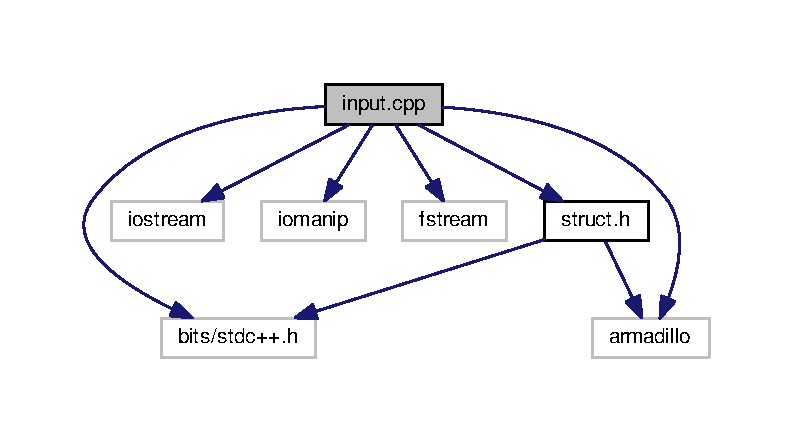
\includegraphics[width=350pt]{input_8cpp__incl}
\end{center}
\end{figure}
This graph shows which files directly or indirectly include this file\+:
\nopagebreak
\begin{figure}[H]
\begin{center}
\leavevmode
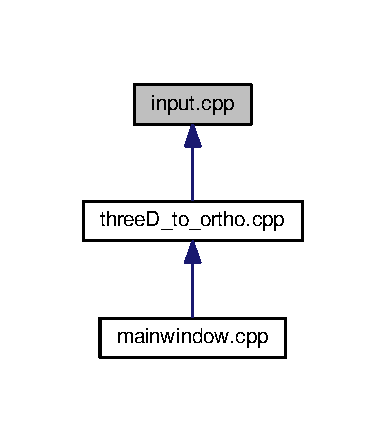
\includegraphics[width=185pt]{input_8cpp__dep__incl}
\end{center}
\end{figure}
\subsection*{Functions}
\begin{DoxyCompactItemize}
\item 
graph \hyperlink{input_8cpp_a0cc06af05bb805fba84d372efc4c247e}{get\+\_\+3\+D\+\_\+graph} (string filename=\char`\"{}input\+\_\+3\+D.\+txt\char`\"{})
\item 
mat \hyperlink{input_8cpp_a80d750ad6a6d88be3e402910c4e7438d}{get\+\_\+mx4\+\_\+matrix} (vector$<$ node $>$ v, int cols=4)
\end{DoxyCompactItemize}


\subsection{Function Documentation}
\mbox{\Hypertarget{input_8cpp_a0cc06af05bb805fba84d372efc4c247e}\label{input_8cpp_a0cc06af05bb805fba84d372efc4c247e}} 
\index{input.\+cpp@{input.\+cpp}!get\+\_\+3\+D\+\_\+graph@{get\+\_\+3\+D\+\_\+graph}}
\index{get\+\_\+3\+D\+\_\+graph@{get\+\_\+3\+D\+\_\+graph}!input.\+cpp@{input.\+cpp}}
\subsubsection{\texorpdfstring{get\+\_\+3\+D\+\_\+graph()}{get\_3D\_graph()}}
{\footnotesize\ttfamily graph get\+\_\+3\+D\+\_\+graph (\begin{DoxyParamCaption}\item[{string}]{filename = {\ttfamily \char`\"{}input\+\_\+3D.txt\char`\"{}} }\end{DoxyParamCaption})}

Reads the 3D input from a file given as an argument. Converts the input into a graph and returns the graph.\mbox{\Hypertarget{input_8cpp_a80d750ad6a6d88be3e402910c4e7438d}\label{input_8cpp_a80d750ad6a6d88be3e402910c4e7438d}} 
\index{input.\+cpp@{input.\+cpp}!get\+\_\+mx4\+\_\+matrix@{get\+\_\+mx4\+\_\+matrix}}
\index{get\+\_\+mx4\+\_\+matrix@{get\+\_\+mx4\+\_\+matrix}!input.\+cpp@{input.\+cpp}}
\subsubsection{\texorpdfstring{get\+\_\+mx4\+\_\+matrix()}{get\_mx4\_matrix()}}
{\footnotesize\ttfamily mat get\+\_\+mx4\+\_\+matrix (\begin{DoxyParamCaption}\item[{vector$<$ node $>$}]{v,  }\item[{int}]{cols = {\ttfamily 4} }\end{DoxyParamCaption})}

Takes a graph as an input. Converts the graph into a 4\+X4 coordinate matrix as specified in the mathematical model.
\hypertarget{main_8cpp}{}\section{main.\+cpp File Reference}
\label{main_8cpp}\index{main.\+cpp@{main.\+cpp}}
{\ttfamily \#include \char`\"{}include/mainwindow.\+h\char`\"{}}\newline
{\ttfamily \#include $<$Q\+Application$>$}\newline
Include dependency graph for main.\+cpp\+:
\nopagebreak
\begin{figure}[H]
\begin{center}
\leavevmode
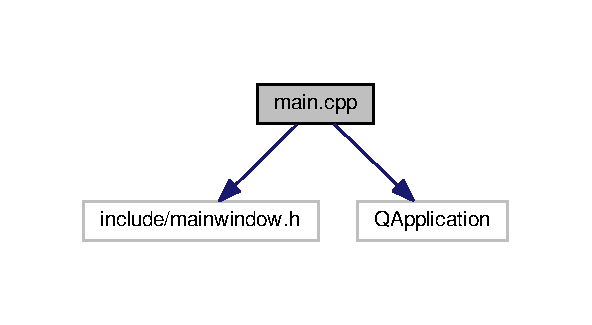
\includegraphics[width=284pt]{main_8cpp__incl}
\end{center}
\end{figure}
\subsection*{Functions}
\begin{DoxyCompactItemize}
\item 
int \hyperlink{main_8cpp_a0ddf1224851353fc92bfbff6f499fa97}{main} (int argc, char $\ast$argv\mbox{[}$\,$\mbox{]})
\end{DoxyCompactItemize}


\subsection{Function Documentation}
\mbox{\Hypertarget{main_8cpp_a0ddf1224851353fc92bfbff6f499fa97}\label{main_8cpp_a0ddf1224851353fc92bfbff6f499fa97}} 
\index{main.\+cpp@{main.\+cpp}!main@{main}}
\index{main@{main}!main.\+cpp@{main.\+cpp}}
\subsubsection{\texorpdfstring{main()}{main()}}
{\footnotesize\ttfamily int main (\begin{DoxyParamCaption}\item[{int}]{argc,  }\item[{char $\ast$}]{argv\mbox{[}$\,$\mbox{]} }\end{DoxyParamCaption})}


\hypertarget{mainwindow_8cpp}{}\section{mainwindow.\+cpp File Reference}
\label{mainwindow_8cpp}\index{mainwindow.\+cpp@{mainwindow.\+cpp}}
{\ttfamily \#include \char`\"{}mainwindow.\+h\char`\"{}}\newline
{\ttfamily \#include $<$ui\+\_\+mainwindow.\+h$>$}\newline
{\ttfamily \#include $<$bits/stdc++.\+h$>$}\newline
{\ttfamily \#include $<$Qt\+Core$>$}\newline
{\ttfamily \#include $<$Qt\+Gui$>$}\newline
{\ttfamily \#include $<$Q\+Label$>$}\newline
{\ttfamily \#include $<$armadillo$>$}\newline
{\ttfamily \#include \char`\"{}draw.\+cpp\char`\"{}}\newline
{\ttfamily \#include \char`\"{}three\+D\+\_\+to\+\_\+ortho.\+cpp\char`\"{}}\newline
{\ttfamily \#include \char`\"{}two\+D\+\_\+to3\+D.\+cpp\char`\"{}}\newline
Include dependency graph for mainwindow.\+cpp\+:
\nopagebreak
\begin{figure}[H]
\begin{center}
\leavevmode
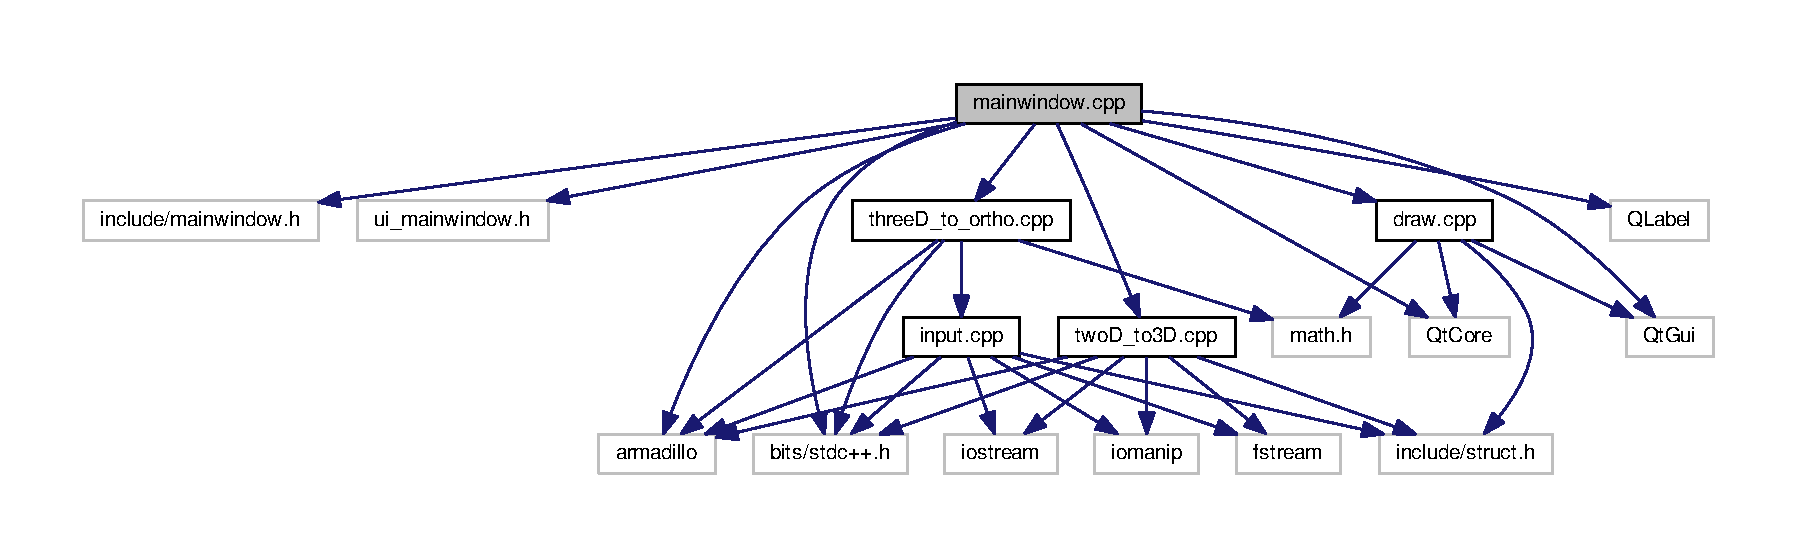
\includegraphics[width=350pt]{mainwindow_8cpp__incl}
\end{center}
\end{figure}
\subsection*{Functions}
\begin{DoxyCompactItemize}
\item 
\hyperlink{structcoordinate}{coordinate} \hyperlink{mainwindow_8cpp_ac71fa7064fdbddf1399ad6cc46ec6091}{add\+\_\+coord} (\hyperlink{structcoordinate}{coordinate} c1, \hyperlink{structcoordinate}{coordinate} c2)
\item 
void \hyperlink{mainwindow_8cpp_abce1fb4bd14a1bd3eefd68ae6aba1ac9}{translate\+\_\+graph} (vector$<$ \hyperlink{structnode}{node} $>$ \&v, \hyperlink{structcoordinate}{coordinate} c)
\end{DoxyCompactItemize}
\subsection*{Variables}
\begin{DoxyCompactItemize}
\item 
vector$<$ \hyperlink{structnode}{node} $>$ \hyperlink{mainwindow_8cpp_aa6e24f1884cfd5ab7e958502b7bdfc9c}{node\+\_\+0}
\item 
vector$<$ \hyperlink{structnode}{node} $>$ \hyperlink{mainwindow_8cpp_a4669e1732c1b71378283bd700c9ea947}{node\+\_\+1}
\item 
vector$<$ \hyperlink{structpair__}{pair\+\_\+} $>$ \hyperlink{mainwindow_8cpp_aced65cd5401c7676b35463d289953b02}{edge\+\_\+codes\+\_\+1}
\item 
int \hyperlink{mainwindow_8cpp_a1ea5d0cb93f22f7d0fdf804bd68c3326}{mode}
\end{DoxyCompactItemize}


\subsection{Function Documentation}
\mbox{\Hypertarget{mainwindow_8cpp_ac71fa7064fdbddf1399ad6cc46ec6091}\label{mainwindow_8cpp_ac71fa7064fdbddf1399ad6cc46ec6091}} 
\index{mainwindow.\+cpp@{mainwindow.\+cpp}!add\+\_\+coord@{add\+\_\+coord}}
\index{add\+\_\+coord@{add\+\_\+coord}!mainwindow.\+cpp@{mainwindow.\+cpp}}
\subsubsection{\texorpdfstring{add\+\_\+coord()}{add\_coord()}}
{\footnotesize\ttfamily \hyperlink{structcoordinate}{coordinate} add\+\_\+coord (\begin{DoxyParamCaption}\item[{\hyperlink{structcoordinate}{coordinate}}]{c1,  }\item[{\hyperlink{structcoordinate}{coordinate}}]{c2 }\end{DoxyParamCaption})}

Helper func that adds two coordinates\mbox{\Hypertarget{mainwindow_8cpp_abce1fb4bd14a1bd3eefd68ae6aba1ac9}\label{mainwindow_8cpp_abce1fb4bd14a1bd3eefd68ae6aba1ac9}} 
\index{mainwindow.\+cpp@{mainwindow.\+cpp}!translate\+\_\+graph@{translate\+\_\+graph}}
\index{translate\+\_\+graph@{translate\+\_\+graph}!mainwindow.\+cpp@{mainwindow.\+cpp}}
\subsubsection{\texorpdfstring{translate\+\_\+graph()}{translate\_graph()}}
{\footnotesize\ttfamily void translate\+\_\+graph (\begin{DoxyParamCaption}\item[{vector$<$ \hyperlink{structnode}{node} $>$ \&}]{v,  }\item[{\hyperlink{structcoordinate}{coordinate}}]{c }\end{DoxyParamCaption})}

Translates graph taking a vector of nodes and an average coordinate

\subsection{Variable Documentation}
\mbox{\Hypertarget{mainwindow_8cpp_aced65cd5401c7676b35463d289953b02}\label{mainwindow_8cpp_aced65cd5401c7676b35463d289953b02}} 
\index{mainwindow.\+cpp@{mainwindow.\+cpp}!edge\+\_\+codes\+\_\+1@{edge\+\_\+codes\+\_\+1}}
\index{edge\+\_\+codes\+\_\+1@{edge\+\_\+codes\+\_\+1}!mainwindow.\+cpp@{mainwindow.\+cpp}}
\subsubsection{\texorpdfstring{edge\+\_\+codes\+\_\+1}{edge\_codes\_1}}
{\footnotesize\ttfamily vector$<$\hyperlink{structpair__}{pair\+\_\+}$>$ edge\+\_\+codes\+\_\+1}

\mbox{\Hypertarget{mainwindow_8cpp_a1ea5d0cb93f22f7d0fdf804bd68c3326}\label{mainwindow_8cpp_a1ea5d0cb93f22f7d0fdf804bd68c3326}} 
\index{mainwindow.\+cpp@{mainwindow.\+cpp}!mode@{mode}}
\index{mode@{mode}!mainwindow.\+cpp@{mainwindow.\+cpp}}
\subsubsection{\texorpdfstring{mode}{mode}}
{\footnotesize\ttfamily int mode}

\mbox{\Hypertarget{mainwindow_8cpp_aa6e24f1884cfd5ab7e958502b7bdfc9c}\label{mainwindow_8cpp_aa6e24f1884cfd5ab7e958502b7bdfc9c}} 
\index{mainwindow.\+cpp@{mainwindow.\+cpp}!node\+\_\+0@{node\+\_\+0}}
\index{node\+\_\+0@{node\+\_\+0}!mainwindow.\+cpp@{mainwindow.\+cpp}}
\subsubsection{\texorpdfstring{node\+\_\+0}{node\_0}}
{\footnotesize\ttfamily vector$<$\hyperlink{structnode}{node}$>$ node\+\_\+0}

\mbox{\Hypertarget{mainwindow_8cpp_a4669e1732c1b71378283bd700c9ea947}\label{mainwindow_8cpp_a4669e1732c1b71378283bd700c9ea947}} 
\index{mainwindow.\+cpp@{mainwindow.\+cpp}!node\+\_\+1@{node\+\_\+1}}
\index{node\+\_\+1@{node\+\_\+1}!mainwindow.\+cpp@{mainwindow.\+cpp}}
\subsubsection{\texorpdfstring{node\+\_\+1}{node\_1}}
{\footnotesize\ttfamily vector$<$\hyperlink{structnode}{node}$>$ node\+\_\+1}


\hypertarget{threeD__to__ortho_8cpp}{}\section{three\+D\+\_\+to\+\_\+ortho.\+cpp File Reference}
\label{threeD__to__ortho_8cpp}\index{three\+D\+\_\+to\+\_\+ortho.\+cpp@{three\+D\+\_\+to\+\_\+ortho.\+cpp}}
{\ttfamily \#include $<$bits/stdc++.\+h$>$}\newline
{\ttfamily \#include $<$armadillo$>$}\newline
{\ttfamily \#include \char`\"{}input.\+cpp\char`\"{}}\newline
{\ttfamily \#include $<$math.\+h$>$}\newline
Include dependency graph for three\+D\+\_\+to\+\_\+ortho.\+cpp\+:
\nopagebreak
\begin{figure}[H]
\begin{center}
\leavevmode
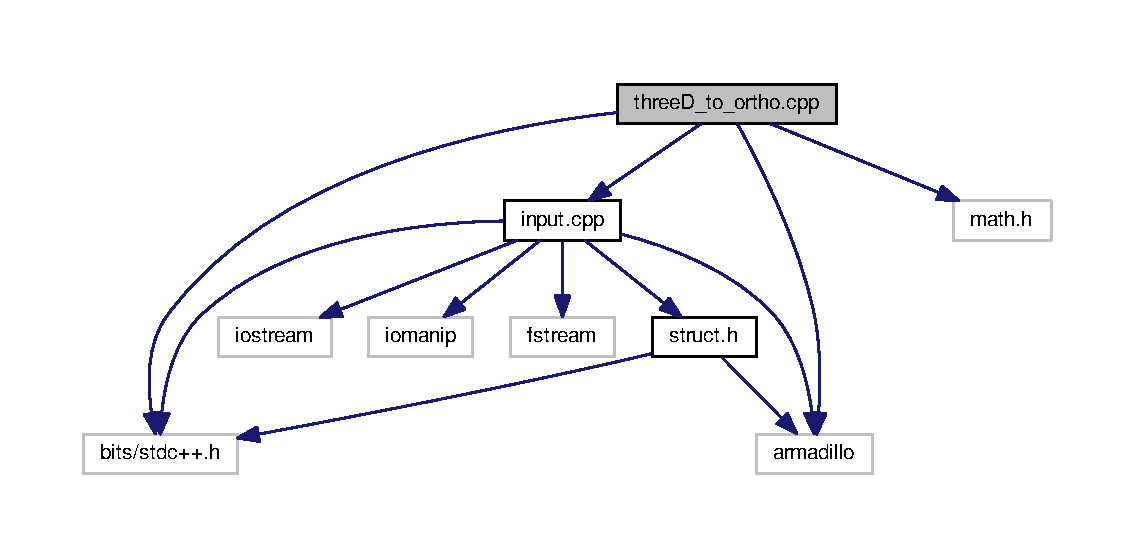
\includegraphics[width=350pt]{threeD__to__ortho_8cpp__incl}
\end{center}
\end{figure}
This graph shows which files directly or indirectly include this file\+:
\nopagebreak
\begin{figure}[H]
\begin{center}
\leavevmode
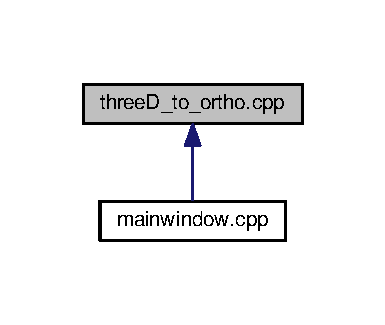
\includegraphics[width=185pt]{threeD__to__ortho_8cpp__dep__incl}
\end{center}
\end{figure}
\subsection*{Macros}
\begin{DoxyCompactItemize}
\item 
\#define \hyperlink{threeD__to__ortho_8cpp_a598a3330b3c21701223ee0ca14316eca}{PI}~3.\+1415926536
\end{DoxyCompactItemize}
\subsection*{Functions}
\begin{DoxyCompactItemize}
\item 
\hyperlink{structdir__ratios}{dir\+\_\+ratios} \hyperlink{threeD__to__ortho_8cpp_a42f9a16ee1fb5f0b3db37d7025ae8fb4}{get\+\_\+dir\+\_\+ratios} ()
\item 
mat \hyperlink{threeD__to__ortho_8cpp_a8420d58e0454a5d63fdb1d74ef96d270}{graph\+\_\+to\+\_\+mat} (vector$<$ \hyperlink{structnode}{node} $>$ nodes, int cols=4)
\item 
vector$<$ \hyperlink{structnode}{node} $>$ \hyperlink{threeD__to__ortho_8cpp_a6293222d57d26a387793e397a0418b31}{mat\+\_\+to\+\_\+graph} (mat A, vector$<$ \hyperlink{structnode}{node} $>$ vec)
\item 
mat \hyperlink{threeD__to__ortho_8cpp_a0f52d843a3641070bfa5443bcc3966d7}{translate\+\_\+graph} (mat A, \hyperlink{structcoordinate}{coordinate} t\+\_\+factor)
\item 
\hyperlink{structrot__matrix}{rot\+\_\+matrix} \hyperlink{threeD__to__ortho_8cpp_a221fd906c7bf89ca0a820709d0734f23}{rot\+\_\+about\+\_\+coord\+\_\+axis} (\hyperlink{structdirection}{direction} theta)
\item 
mat \hyperlink{threeD__to__ortho_8cpp_acd70b7328b74ddc50dc03870b7e3a6ed}{find\+\_\+rot} (mat A, \hyperlink{structdir__ratios}{dir\+\_\+ratios} d)
\item 
mat \hyperlink{threeD__to__ortho_8cpp_a50ff42487e337cc300dddef30e476cc0}{find\+\_\+projection} (mat A)
\item 
vector$<$ \hyperlink{structnode}{node} $>$ \hyperlink{threeD__to__ortho_8cpp_a3ced4e2119422236523faa8fcdd68acb}{find\+\_\+ortho} (vector$<$ \hyperlink{structnode}{node} $>$ \hyperlink{structgraph}{graph})
\item 
void \hyperlink{threeD__to__ortho_8cpp_a87e17a4e0a3335783284b821f184a923}{rotate\+\_\+graph} (vector$<$ \hyperlink{structnode}{node} $>$ \&v, \hyperlink{structdirection}{direction} theta, int x, int y, int z)
\end{DoxyCompactItemize}


\subsection{Macro Definition Documentation}
\mbox{\Hypertarget{threeD__to__ortho_8cpp_a598a3330b3c21701223ee0ca14316eca}\label{threeD__to__ortho_8cpp_a598a3330b3c21701223ee0ca14316eca}} 
\index{three\+D\+\_\+to\+\_\+ortho.\+cpp@{three\+D\+\_\+to\+\_\+ortho.\+cpp}!PI@{PI}}
\index{PI@{PI}!three\+D\+\_\+to\+\_\+ortho.\+cpp@{three\+D\+\_\+to\+\_\+ortho.\+cpp}}
\subsubsection{\texorpdfstring{PI}{PI}}
{\footnotesize\ttfamily \#define PI~3.\+1415926536}



\subsection{Function Documentation}
\mbox{\Hypertarget{threeD__to__ortho_8cpp_a3ced4e2119422236523faa8fcdd68acb}\label{threeD__to__ortho_8cpp_a3ced4e2119422236523faa8fcdd68acb}} 
\index{three\+D\+\_\+to\+\_\+ortho.\+cpp@{three\+D\+\_\+to\+\_\+ortho.\+cpp}!find\+\_\+ortho@{find\+\_\+ortho}}
\index{find\+\_\+ortho@{find\+\_\+ortho}!three\+D\+\_\+to\+\_\+ortho.\+cpp@{three\+D\+\_\+to\+\_\+ortho.\+cpp}}
\subsubsection{\texorpdfstring{find\+\_\+ortho()}{find\_ortho()}}
{\footnotesize\ttfamily vector$<$\hyperlink{structnode}{node}$>$ find\+\_\+ortho (\begin{DoxyParamCaption}\item[{vector$<$ \hyperlink{structnode}{node} $>$}]{graph }\end{DoxyParamCaption})}

Takes the graph whose projection is required to be taken as an argument. Then asks the user about the direction ratios of the desired line of sight. Then converts the graph to a matrix. Finds the transitions to be done. Applies the transitions to the coordinate matrx. Converts the matrix back to a graph and returns it.\mbox{\Hypertarget{threeD__to__ortho_8cpp_a50ff42487e337cc300dddef30e476cc0}\label{threeD__to__ortho_8cpp_a50ff42487e337cc300dddef30e476cc0}} 
\index{three\+D\+\_\+to\+\_\+ortho.\+cpp@{three\+D\+\_\+to\+\_\+ortho.\+cpp}!find\+\_\+projection@{find\+\_\+projection}}
\index{find\+\_\+projection@{find\+\_\+projection}!three\+D\+\_\+to\+\_\+ortho.\+cpp@{three\+D\+\_\+to\+\_\+ortho.\+cpp}}
\subsubsection{\texorpdfstring{find\+\_\+projection()}{find\_projection()}}
{\footnotesize\ttfamily mat find\+\_\+projection (\begin{DoxyParamCaption}\item[{mat}]{A }\end{DoxyParamCaption})}

Returns the projection of the graph after applying all the required transitions using z axis as the line-\/of-\/sight.\mbox{\Hypertarget{threeD__to__ortho_8cpp_acd70b7328b74ddc50dc03870b7e3a6ed}\label{threeD__to__ortho_8cpp_acd70b7328b74ddc50dc03870b7e3a6ed}} 
\index{three\+D\+\_\+to\+\_\+ortho.\+cpp@{three\+D\+\_\+to\+\_\+ortho.\+cpp}!find\+\_\+rot@{find\+\_\+rot}}
\index{find\+\_\+rot@{find\+\_\+rot}!three\+D\+\_\+to\+\_\+ortho.\+cpp@{three\+D\+\_\+to\+\_\+ortho.\+cpp}}
\subsubsection{\texorpdfstring{find\+\_\+rot()}{find\_rot()}}
{\footnotesize\ttfamily mat find\+\_\+rot (\begin{DoxyParamCaption}\item[{mat}]{A,  }\item[{\hyperlink{structdir__ratios}{dir\+\_\+ratios}}]{d }\end{DoxyParamCaption})}

Takes two inputs
\begin{DoxyItemize}
\item The matrix A which has to translated
\item The direction ratios of the direction which has to become the line of sight for taking the projections. This function calls the function rot\+\_\+about\+\_\+coord\+\_\+axis to get the rotation matrices and then multiplies the matrices with the coordinate matrix. It returns the coordinate matrix after multiplying it with the rotation matrices.
\end{DoxyItemize}\mbox{\Hypertarget{threeD__to__ortho_8cpp_a42f9a16ee1fb5f0b3db37d7025ae8fb4}\label{threeD__to__ortho_8cpp_a42f9a16ee1fb5f0b3db37d7025ae8fb4}} 
\index{three\+D\+\_\+to\+\_\+ortho.\+cpp@{three\+D\+\_\+to\+\_\+ortho.\+cpp}!get\+\_\+dir\+\_\+ratios@{get\+\_\+dir\+\_\+ratios}}
\index{get\+\_\+dir\+\_\+ratios@{get\+\_\+dir\+\_\+ratios}!three\+D\+\_\+to\+\_\+ortho.\+cpp@{three\+D\+\_\+to\+\_\+ortho.\+cpp}}
\subsubsection{\texorpdfstring{get\+\_\+dir\+\_\+ratios()}{get\_dir\_ratios()}}
{\footnotesize\ttfamily \hyperlink{structdir__ratios}{dir\+\_\+ratios} get\+\_\+dir\+\_\+ratios (\begin{DoxyParamCaption}{ }\end{DoxyParamCaption})}

Asks the user for the direction along which it is desired to take the projection.\mbox{\Hypertarget{threeD__to__ortho_8cpp_a8420d58e0454a5d63fdb1d74ef96d270}\label{threeD__to__ortho_8cpp_a8420d58e0454a5d63fdb1d74ef96d270}} 
\index{three\+D\+\_\+to\+\_\+ortho.\+cpp@{three\+D\+\_\+to\+\_\+ortho.\+cpp}!graph\+\_\+to\+\_\+mat@{graph\+\_\+to\+\_\+mat}}
\index{graph\+\_\+to\+\_\+mat@{graph\+\_\+to\+\_\+mat}!three\+D\+\_\+to\+\_\+ortho.\+cpp@{three\+D\+\_\+to\+\_\+ortho.\+cpp}}
\subsubsection{\texorpdfstring{graph\+\_\+to\+\_\+mat()}{graph\_to\_mat()}}
{\footnotesize\ttfamily mat graph\+\_\+to\+\_\+mat (\begin{DoxyParamCaption}\item[{vector$<$ \hyperlink{structnode}{node} $>$}]{nodes,  }\item[{int}]{cols = {\ttfamily 4} }\end{DoxyParamCaption})}

Takes a graph as an input. Converts the graph into a 4\+X4 coordinate matrix as specified in the mathematical model.\mbox{\Hypertarget{threeD__to__ortho_8cpp_a6293222d57d26a387793e397a0418b31}\label{threeD__to__ortho_8cpp_a6293222d57d26a387793e397a0418b31}} 
\index{three\+D\+\_\+to\+\_\+ortho.\+cpp@{three\+D\+\_\+to\+\_\+ortho.\+cpp}!mat\+\_\+to\+\_\+graph@{mat\+\_\+to\+\_\+graph}}
\index{mat\+\_\+to\+\_\+graph@{mat\+\_\+to\+\_\+graph}!three\+D\+\_\+to\+\_\+ortho.\+cpp@{three\+D\+\_\+to\+\_\+ortho.\+cpp}}
\subsubsection{\texorpdfstring{mat\+\_\+to\+\_\+graph()}{mat\_to\_graph()}}
{\footnotesize\ttfamily vector$<$\hyperlink{structnode}{node}$>$ mat\+\_\+to\+\_\+graph (\begin{DoxyParamCaption}\item[{mat}]{A,  }\item[{vector$<$ \hyperlink{structnode}{node} $>$}]{vec }\end{DoxyParamCaption})}

Takes a coordinate matrix as an input. Converts 4\+X4 coordinate matrix to the graph which would lead to constriuction of this matrix.\mbox{\Hypertarget{threeD__to__ortho_8cpp_a221fd906c7bf89ca0a820709d0734f23}\label{threeD__to__ortho_8cpp_a221fd906c7bf89ca0a820709d0734f23}} 
\index{three\+D\+\_\+to\+\_\+ortho.\+cpp@{three\+D\+\_\+to\+\_\+ortho.\+cpp}!rot\+\_\+about\+\_\+coord\+\_\+axis@{rot\+\_\+about\+\_\+coord\+\_\+axis}}
\index{rot\+\_\+about\+\_\+coord\+\_\+axis@{rot\+\_\+about\+\_\+coord\+\_\+axis}!three\+D\+\_\+to\+\_\+ortho.\+cpp@{three\+D\+\_\+to\+\_\+ortho.\+cpp}}
\subsubsection{\texorpdfstring{rot\+\_\+about\+\_\+coord\+\_\+axis()}{rot\_about\_coord\_axis()}}
{\footnotesize\ttfamily \hyperlink{structrot__matrix}{rot\+\_\+matrix} rot\+\_\+about\+\_\+coord\+\_\+axis (\begin{DoxyParamCaption}\item[{\hyperlink{structdirection}{direction}}]{theta }\end{DoxyParamCaption})}

Takes the direction ratios as the input It returns the rotation matrices which are to be multiplied to the coordinate matrix so as to make the Z axis coincide with the given direction theta. It returns a struct of \hyperlink{structrot__matrix}{rot\+\_\+matrix} type which contains the three rotation matrices namely Rx, Ry and Rz.\mbox{\Hypertarget{threeD__to__ortho_8cpp_a87e17a4e0a3335783284b821f184a923}\label{threeD__to__ortho_8cpp_a87e17a4e0a3335783284b821f184a923}} 
\index{three\+D\+\_\+to\+\_\+ortho.\+cpp@{three\+D\+\_\+to\+\_\+ortho.\+cpp}!rotate\+\_\+graph@{rotate\+\_\+graph}}
\index{rotate\+\_\+graph@{rotate\+\_\+graph}!three\+D\+\_\+to\+\_\+ortho.\+cpp@{three\+D\+\_\+to\+\_\+ortho.\+cpp}}
\subsubsection{\texorpdfstring{rotate\+\_\+graph()}{rotate\_graph()}}
{\footnotesize\ttfamily void rotate\+\_\+graph (\begin{DoxyParamCaption}\item[{vector$<$ \hyperlink{structnode}{node} $>$ \&}]{v,  }\item[{\hyperlink{structdirection}{direction}}]{theta,  }\item[{int}]{x,  }\item[{int}]{y,  }\item[{int}]{z }\end{DoxyParamCaption})}

Rotate the given graph about axis (X, Y or Z axis) depending on the input x, y and z Finsd the rotations matrix for the given direction theta and applies only those whose corresponding input is 1. For Rx, x is to be 1. For Ry, y is to be 1. For Rz, z is to be 1.\mbox{\Hypertarget{threeD__to__ortho_8cpp_a0f52d843a3641070bfa5443bcc3966d7}\label{threeD__to__ortho_8cpp_a0f52d843a3641070bfa5443bcc3966d7}} 
\index{three\+D\+\_\+to\+\_\+ortho.\+cpp@{three\+D\+\_\+to\+\_\+ortho.\+cpp}!translate\+\_\+graph@{translate\+\_\+graph}}
\index{translate\+\_\+graph@{translate\+\_\+graph}!three\+D\+\_\+to\+\_\+ortho.\+cpp@{three\+D\+\_\+to\+\_\+ortho.\+cpp}}
\subsubsection{\texorpdfstring{translate\+\_\+graph()}{translate\_graph()}}
{\footnotesize\ttfamily mat translate\+\_\+graph (\begin{DoxyParamCaption}\item[{mat}]{A,  }\item[{\hyperlink{structcoordinate}{coordinate}}]{t\+\_\+factor }\end{DoxyParamCaption})}

Takes two inputs
\begin{DoxyItemize}
\item The matrix A (for the corresponding graph) which has to translated
\item The coordinate t\+\_\+factor of the point that would become the origin in the translated system. This function makes multiple calls to the function translate\+\_\+coordinate for all the vertices of the input graph.
\end{DoxyItemize}
\hypertarget{twoD__to3D_8cpp}{}\section{two\+D\+\_\+to3\+D.\+cpp File Reference}
\label{twoD__to3D_8cpp}\index{two\+D\+\_\+to3\+D.\+cpp@{two\+D\+\_\+to3\+D.\+cpp}}
{\ttfamily \#include $<$bits/stdc++.\+h$>$}\newline
{\ttfamily \#include $<$iostream$>$}\newline
{\ttfamily \#include $<$iomanip$>$}\newline
{\ttfamily \#include $<$fstream$>$}\newline
{\ttfamily \#include $<$armadillo$>$}\newline
{\ttfamily \#include \char`\"{}struct.\+h\char`\"{}}\newline
Include dependency graph for two\+D\+\_\+to3\+D.\+cpp\+:
\nopagebreak
\begin{figure}[H]
\begin{center}
\leavevmode
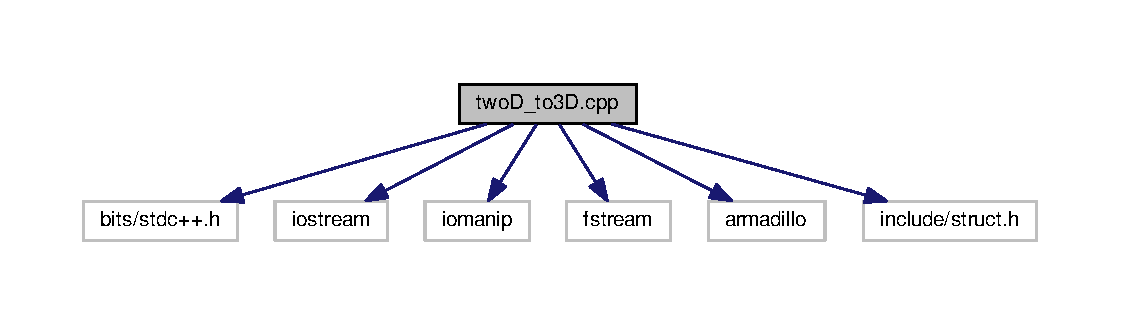
\includegraphics[width=350pt]{twoD__to3D_8cpp__incl}
\end{center}
\end{figure}
This graph shows which files directly or indirectly include this file\+:
\nopagebreak
\begin{figure}[H]
\begin{center}
\leavevmode
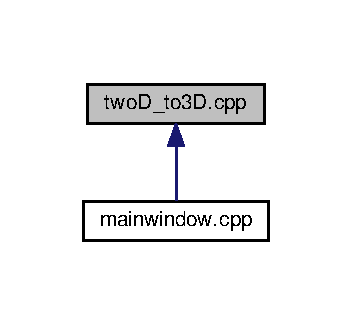
\includegraphics[width=169pt]{twoD__to3D_8cpp__dep__incl}
\end{center}
\end{figure}
\subsection*{Functions}
\begin{DoxyCompactItemize}
\item 
vector$<$ \hyperlink{structnode}{node} $>$ \hyperlink{twoD__to3D_8cpp_ab227b999265cfd25b8de2ed7849b44ec}{get\+\_\+2\+D\+\_\+graph} (string filename)
\item 
vector$<$ \hyperlink{structpair__}{pair\+\_\+} $>$ \hyperlink{twoD__to3D_8cpp_aa5a4d7bb445505454118a3e5972556cc}{get\+\_\+pair\+\_\+2D} (string filename)
\item 
void \hyperlink{twoD__to3D_8cpp_a0653f9d40a0a80b4296347e603c68f06}{check\+\_\+graph} (vector$<$ \hyperlink{structnode}{node} $>$ v)
\end{DoxyCompactItemize}


\subsection{Function Documentation}
\mbox{\Hypertarget{twoD__to3D_8cpp_a0653f9d40a0a80b4296347e603c68f06}\label{twoD__to3D_8cpp_a0653f9d40a0a80b4296347e603c68f06}} 
\index{two\+D\+\_\+to3\+D.\+cpp@{two\+D\+\_\+to3\+D.\+cpp}!check\+\_\+graph@{check\+\_\+graph}}
\index{check\+\_\+graph@{check\+\_\+graph}!two\+D\+\_\+to3\+D.\+cpp@{two\+D\+\_\+to3\+D.\+cpp}}
\subsubsection{\texorpdfstring{check\+\_\+graph()}{check\_graph()}}
{\footnotesize\ttfamily void check\+\_\+graph (\begin{DoxyParamCaption}\item[{vector$<$ \hyperlink{structnode}{node} $>$}]{v }\end{DoxyParamCaption})}

\mbox{\Hypertarget{twoD__to3D_8cpp_ab227b999265cfd25b8de2ed7849b44ec}\label{twoD__to3D_8cpp_ab227b999265cfd25b8de2ed7849b44ec}} 
\index{two\+D\+\_\+to3\+D.\+cpp@{two\+D\+\_\+to3\+D.\+cpp}!get\+\_\+2\+D\+\_\+graph@{get\+\_\+2\+D\+\_\+graph}}
\index{get\+\_\+2\+D\+\_\+graph@{get\+\_\+2\+D\+\_\+graph}!two\+D\+\_\+to3\+D.\+cpp@{two\+D\+\_\+to3\+D.\+cpp}}
\subsubsection{\texorpdfstring{get\+\_\+2\+D\+\_\+graph()}{get\_2D\_graph()}}
{\footnotesize\ttfamily vector$<$\hyperlink{structnode}{node}$>$ get\+\_\+2\+D\+\_\+graph (\begin{DoxyParamCaption}\item[{string}]{filename }\end{DoxyParamCaption})}

Reads the 2D input from a file given as an argument. Converts the input into a graph and returns the graph.\mbox{\Hypertarget{twoD__to3D_8cpp_aa5a4d7bb445505454118a3e5972556cc}\label{twoD__to3D_8cpp_aa5a4d7bb445505454118a3e5972556cc}} 
\index{two\+D\+\_\+to3\+D.\+cpp@{two\+D\+\_\+to3\+D.\+cpp}!get\+\_\+pair\+\_\+2D@{get\+\_\+pair\+\_\+2D}}
\index{get\+\_\+pair\+\_\+2D@{get\+\_\+pair\+\_\+2D}!two\+D\+\_\+to3\+D.\+cpp@{two\+D\+\_\+to3\+D.\+cpp}}
\subsubsection{\texorpdfstring{get\+\_\+pair\+\_\+2\+D()}{get\_pair\_2D()}}
{\footnotesize\ttfamily vector$<$\hyperlink{structpair__}{pair\+\_\+}$>$ get\+\_\+pair\+\_\+2D (\begin{DoxyParamCaption}\item[{string}]{filename }\end{DoxyParamCaption})}

Reads the 2D input from a file given as an argument. Returns all pairs of vertices that have an edge between them according to the input in the file.
%--- End generated contents ---

% Index
\backmatter
\newpage
\phantomsection
\clearemptydoublepage
\addcontentsline{toc}{chapter}{Index}
\printindex

\end{document}
